\chapter{Méthodes de calcul}\label{chap:metho}

Tu diagonalise dans le fond. Et aussi tu fixes parfois des conditions de frontière. What if I add on another phrase?

Ahh et aussi,
\al{
    \int_{a}^{b} f(x)\,\symup{d}x = F(b) - F(a)
}
Et pour un vecteur maintenant:
\al{
\symbf{a}\cdot\symbf{b}\label{eq:dot_product}
}
$\mathcal{R}\mathscr{R}\mathfrak{R}\mathbb{R}\mathbb{C}f$

The quick brown fox jumps over the lazy dog. The quick brown fox jumps over the lazy dog. The quick brown fox jumps over the lazy dog. The quick brown fox jumps over the lazy dog. The quick brown fox jumps over the lazy dog. The quick brown fox jumps over the lazy dog. The quick brown fox jumps over the lazy dog. The quick brown fox jumps over the lazy dog.

The quick brown fox jumps over the lazy dog. The quick brown fox jumps over the lazy dog. The quick brown fox jumps over the lazy dog. The quick brown fox jumps over the lazy dog. The quick brown fox jumps over the lazy dog. The quick brown fox jumps over the lazy dog. The quick brown fox jumps over the lazy dog. The quick brown fox jumps over the lazy dog. The quick brown fox jumps over the lazy dog.

The quick brown fox jumps over the lazy dog.

BTW, this is just the dot product \eqref{eq:dot_product}. This is a woodcock \ref{fig:Estoopi_bird}

\begin{figure}[H]
	\centering
	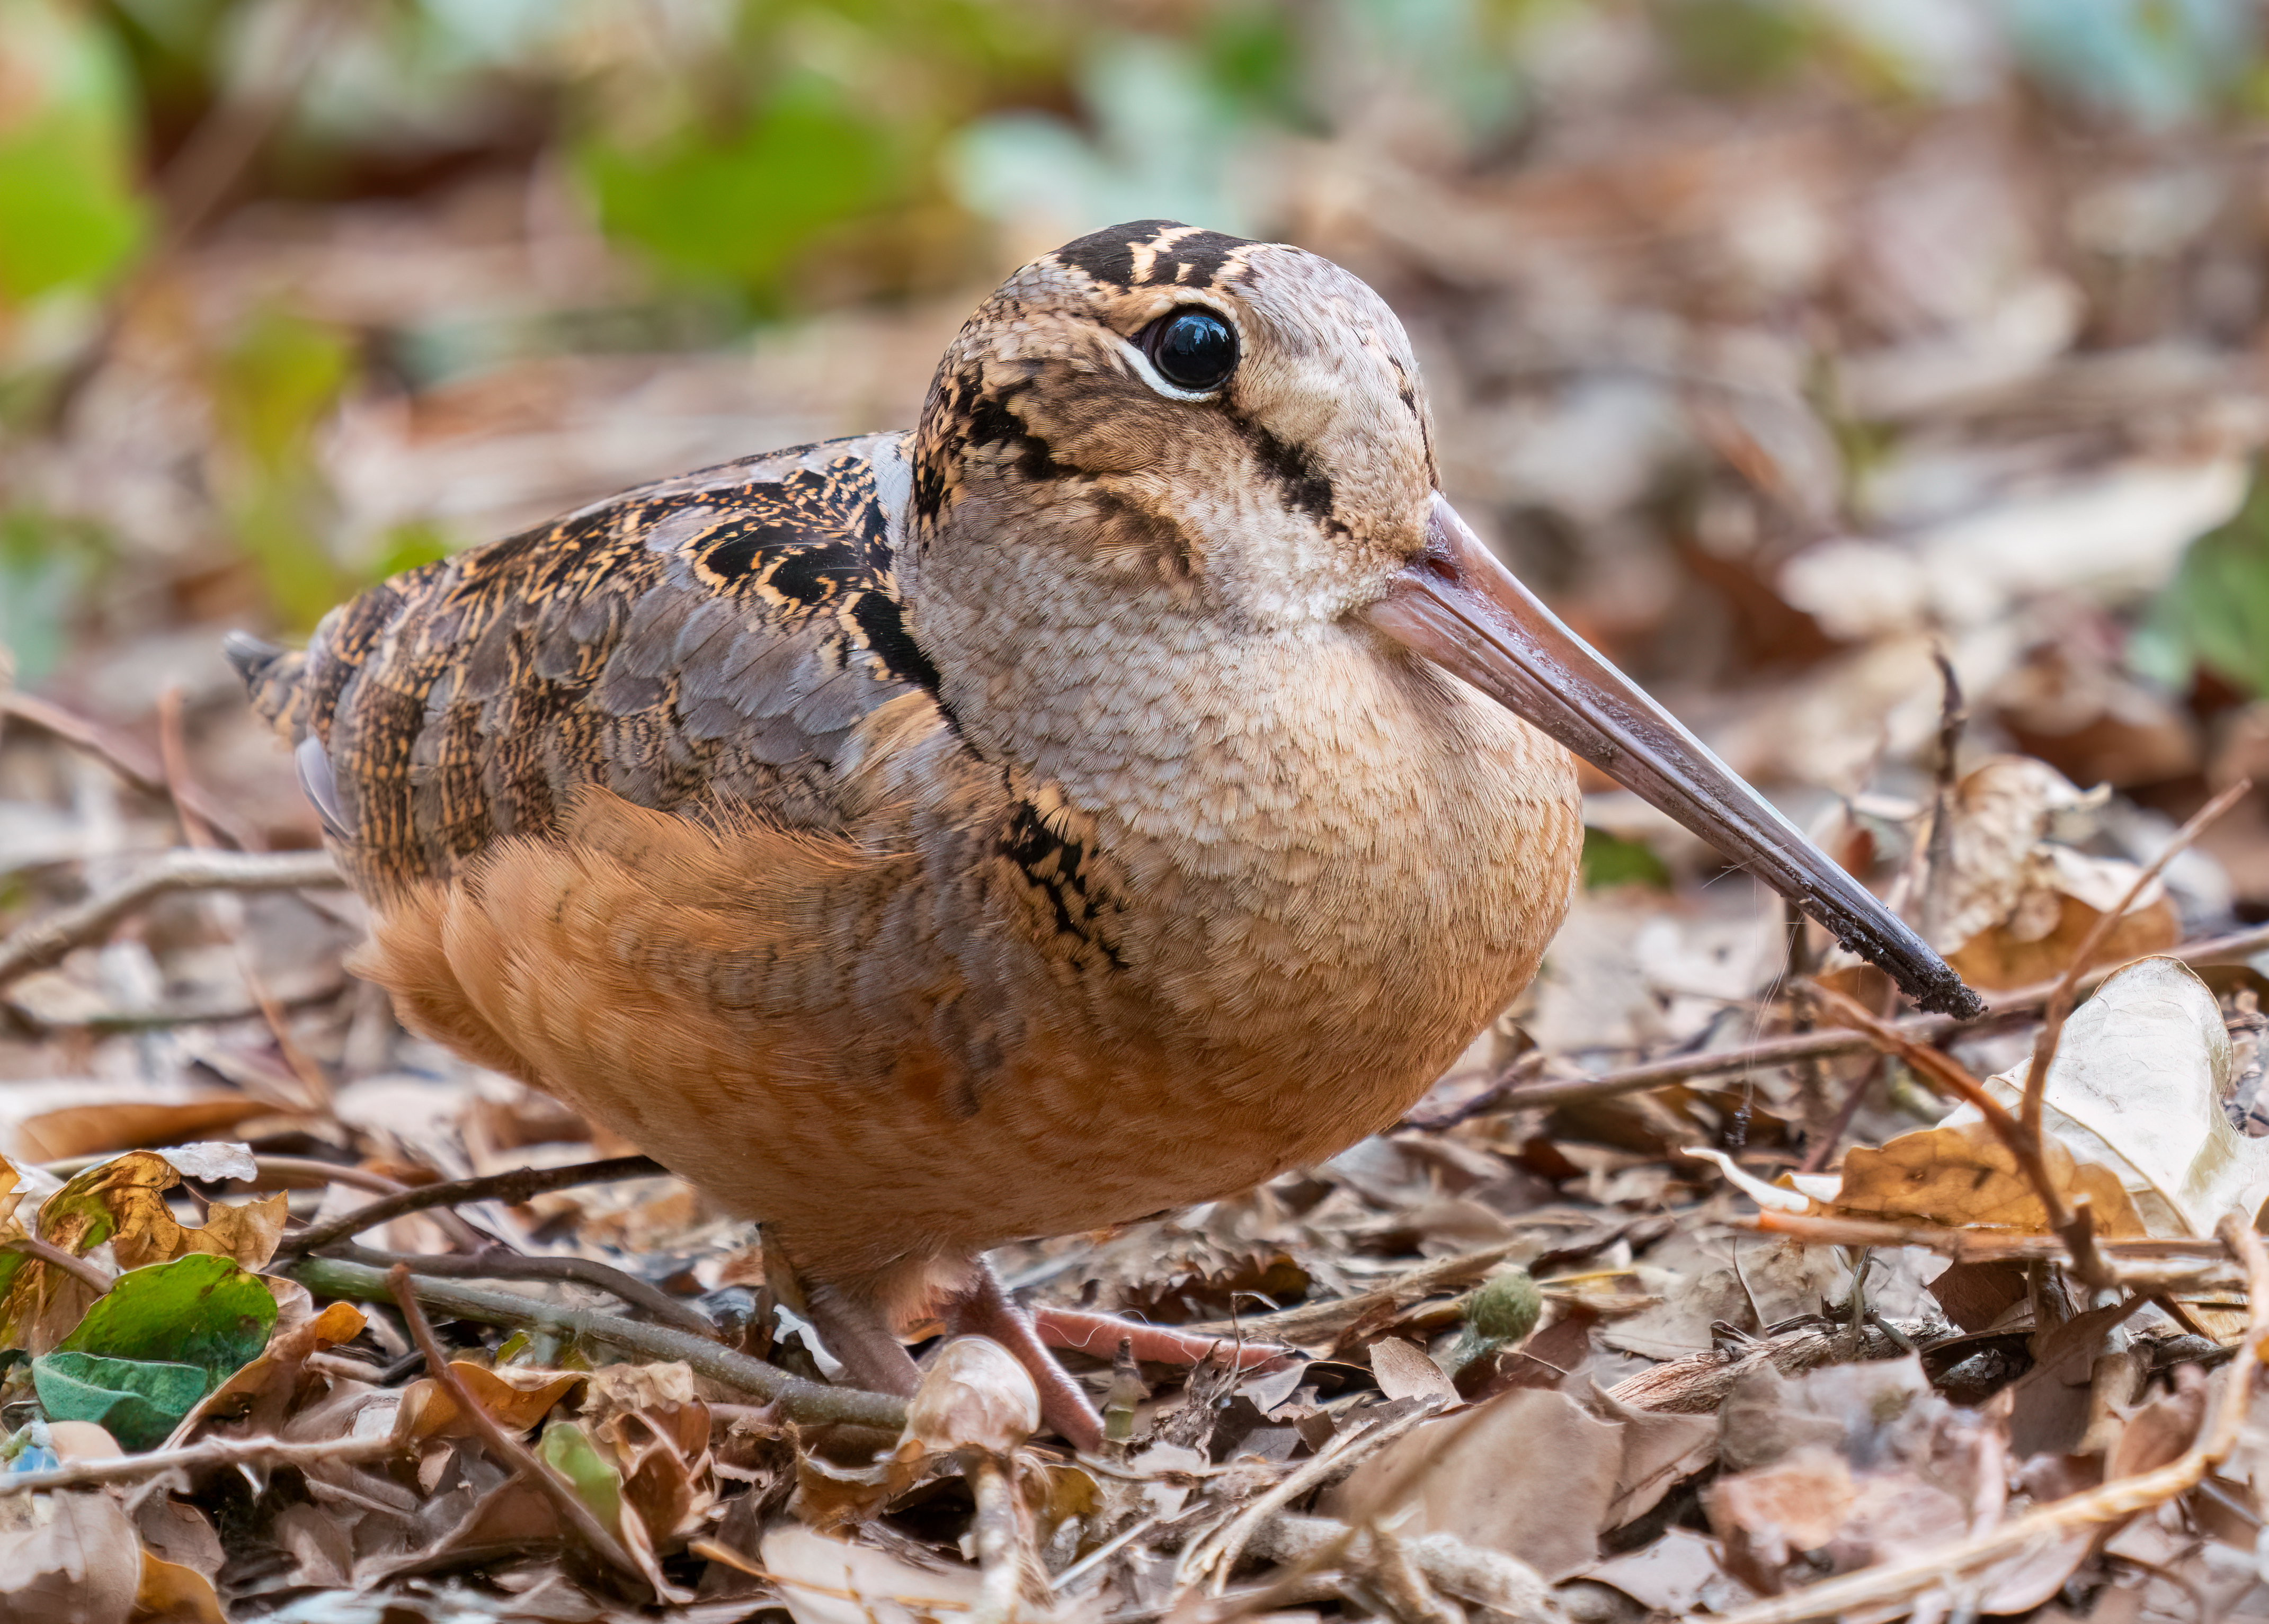
\includegraphics[width=0.5\textwidth]{figures/American_woodcock.jpg}
	\caption{Une bécasse d'Amérique. Un \enquote*{\emph{stoopi-bird}} certifié. En Français, on dit un \enquote{\emph{Oisot}}}
	\label{fig:Estoopi_bird}
\end{figure}

This is nabla $\nabla$. Now this is $\symbf{\nabla}$. How about $\beta$? And now $\symbf{\beta}$... scary!

Now, let $\ve{v}\in\mathbb{R}$

The Wilson loop operator reads as:
\al{
    \boxed{
        \op{W} = \mathcal{T}\Exp{-\oint\D\op{A}}
    }
}
where a creation or annihilation operator would look like $\op{c}_\alpha$ or $\op{c}^\dag_\beta$. Here is just a dagger ($\dagger$) and a double dagger ($\ddagger$). Hence, a general hamiltonian will look like:
\al{
    \op{H} = \sum_{\mu\nu}t_{\mu\nu}\op{c}_\mu^\dagger\op{c}_\nu + \sum_{\alpha\beta\mu\nu}V_{\alpha\beta\mu\nu}\op{c}^\dagger_\alpha\op{c}^\dagger_\beta\op{c}_\mu\op{c}_\nu
}
At equilibrium we say that:
\begin{empheq}[box=\fcolorbox{MainColor}{white}]{equation}
    \op{H} = \sum_{\mu\nu}t_{\mu\nu}\op{c}_\mu^\dagger\op{c}_\nu + \sum_{\alpha\beta\mu\nu}V_{\alpha\beta\mu\nu}\op{c}^\dagger_\alpha\op{c}^\dagger_\beta\op{c}_\mu\op{c}_\nu
\end{empheq}
Let's try this:
\eqn{\cboxed{
    \ve{F} = \dd[p]{t}
}}
Which would be used in the following way normally:
\al{
    \delta S[\phi]=0 ~\Longleftrightarrow~ \cboxed{\ddf[\mathcal{L}]{\phi(x)} - \partial_{\mu}\ddf[\mathcal{L}]{\partial_{\mu}\phi(x)}}
}
Now testing derivatives
\al{
    \dd[f]{x}[2]
}
\begin{theorembox}{Summation of Numbers}{summation}
  Pour tout $n\in\mathbb{N}$,
  \begin{equation}
    \sum_{i=1}^{n} i  = \frac{n\p{n+1}}{2}.
  \end{equation}
  C'est un résultat souvent attribué au jeune Gauss.
\end{theorembox}

\begin{definitionbox}{Goofy Birb}{goofy}
    Un \enquote{Goofy Birb} est défini comme étant un birb qui est excessivement \emph{pomp}.
\end{definitionbox}
